\documentclass[13pt]{memoir}
\setulmarginsandblock{2cm}{2cm}{*}
\setlrmarginsandblock{1.5cm}{1.5cm}{*}
\checkandfixthelayout
\usepackage[spanish,activeacute,es-tabla]{babel}
\usepackage{amsmath}
\usepackage{amssymb,latexsym}
\usepackage[spanish]{layout}
\usepackage{graphicx} 
\usepackage{bigints}
\usepackage{hyperref} 
\usepackage[utf8]{inputenc}

\begin{document}

\begin{center}
			\centering
			Actividad No. $(2)$\\
			$2024$ Cálculo Vectorial.\\
			Nombres:  Camilo Rivera, Emerson Tavera, Karen Torres
\end{center}

\begin{enumerate}

\item[ 1] Diga si la afirmación es verdadera o falsa. Justifique sus respuestas: 
	
	
	
	\item[ a)] La gráfica del dominio de $f(x, y) = \ln(9x^2 - y^2 - 9)$ \\
	\begin{center}
	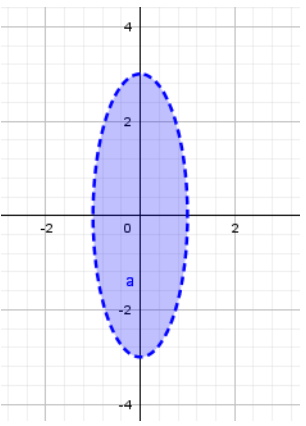
\includegraphics[scale=1]{assets/t_2_1.png} 
	\end{center}
	
	R// Falso\\
	\text{Pues Dada la función: } $f(x, y) = \ln(9x^2 - y^2 - 9)$ \\
	$9x^2 - y^2 - 9 > 0$\\
	$9x^2 - y^2 > 9$\\
	$x^2 - \frac{y^2}{9} > 1$\\ 
	
	lo que representado gráficamente es:
	\begin{center}
	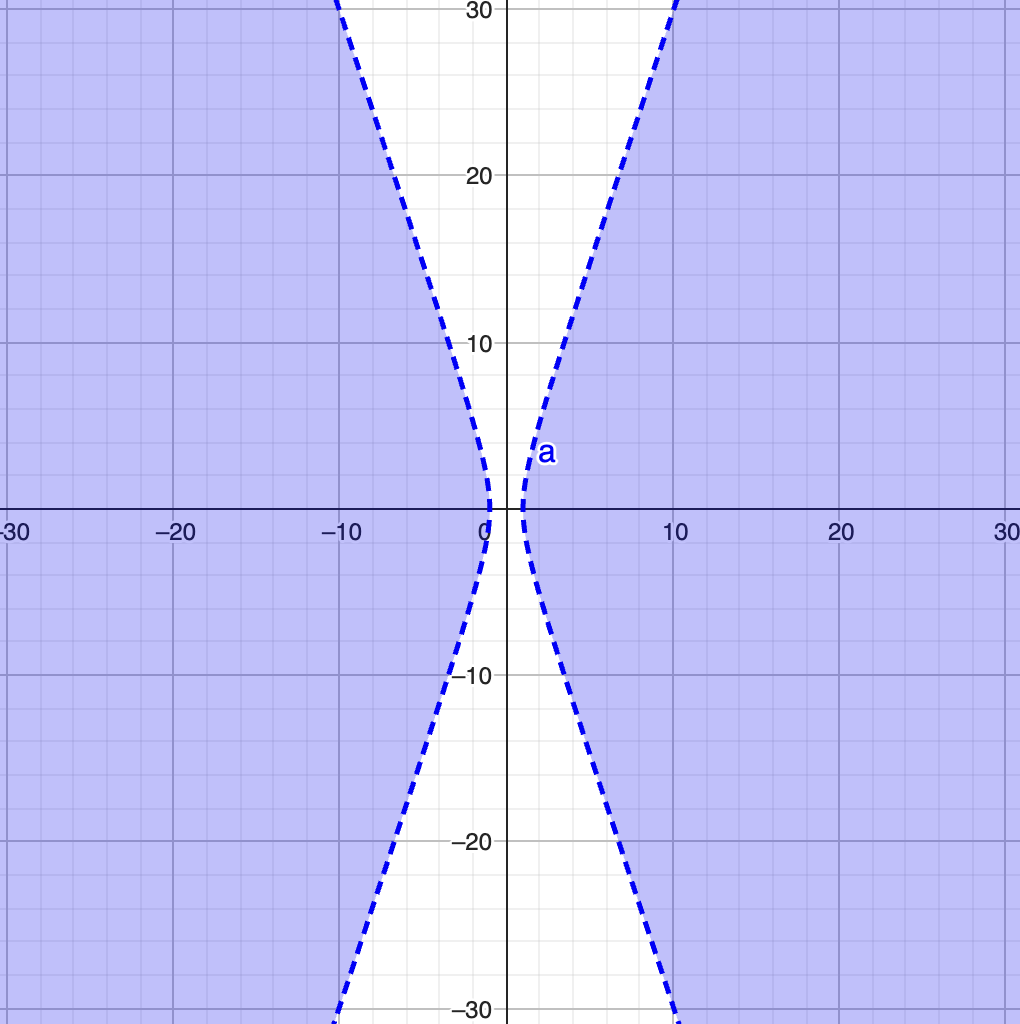
\includegraphics[scale=0.3]{assets/t_2_2.png} 
	\end{center}
	
	
\item[ b)] $F_{xx} = \frac{1}{2\cos(x)}; \;Si\;  f(x, y) = \int_y^x \ln(\cos(t)) \, dt.$ \\
	
$f(x, y) = \int_y^x \ln(\cos(t)) \, dt $ \\

{\tiny \(f_x\) teorema fundamental del cálculo}\\
$f_x = \frac{\partial}{\partial x} \int_y^x \ln(\cos(t)) \, dt = \ln(\cos(x))$\\

{\tiny\(f_{xx}\)  regla de la cadena para diferenciar \(f_x\) con respecto a \(x\):}\\
$f_{xx} = \frac{d}{dx} \ln(\cos(x)) = \frac{1}{\cos(x)} \cdot (-\sin(x)) = -\tan(x)$\\

\textbf{ R// Falso} $f_{xx} = -\tan(x) \neq \frac{1}{2\cos(x)}$\\

\item[ c)] $F_{yy} = \frac{y}{\cos(y)}; \; Si \;f(x, y) = \frac{\sin(x+y)}{x} $ \\

$\frac{\partial \:}{\partial \:y}\left(\frac{\sin \left(x+y\right)}{x}\right) = \frac{1}{x}\frac{\partial \:}{\partial \:y}\left(\sin \left(x+y\right)\right)$\\

{\tiny Regla cadena}\\
$\frac{\partial \:}{\partial \:u}\left(\sin \left(u\right)\right)\frac{\partial \:}{\partial \:y}\left(x+y\right) = \cos \left(u\right)\frac{\partial \:}{\partial \:y}\left(x+y\right) = $ \\
$\cos \left(x+y\right)\frac{\partial \:}{\partial \:y}\left(x+y\right)$\\
$\frac{\partial \:}{\partial \:y}\left(x\right)+\frac{\partial \:}{\partial \:y}\left(y\right) = 0 + 1$\\
$\frac{1}{x}\cos \left(x+y\right)\cdot \:1 =\frac{\cos \left(x+y\right)}{x}$\\

$\frac{\partial \:}{\partial \:y}\left(\frac{\cos \left(x+y\right)}{x}\right) =\frac{1}{x}\frac{\partial \:}{\partial \:y}\left(\cos \left(x+y\right)\right)$

{\tiny Regla cadena}\\
$\frac{\partial \:}{\partial \:y}\left(\cos \left(x+y\right)\right)$\\
$\frac{\partial \:}{\partial \:u}\left(\cos \left(u\right)\right)\frac{\partial \:}{\partial \:y}\left(x+y\right)=$\\
$-\sin \left(u\right)\frac{\partial \:}{\partial \:y}\left(x+y\right)=$\\
$-\sin \left(x+y\right)\frac{\partial \:}{\partial \:y}\left(x+y\right)$\\
$=\frac{1}{x}\left(-\sin \left(x+y\right)\cdot \:1\right) = -\frac{\sin \left(x+y\right)}{x}$\\

\textbf{ R// Falso} $-\frac{\sin \left(x+y\right)}{x} \neq \frac{\sin \left(x+y\right)}{x} $\\

\item[ D)] $F_{yx} = F_{xy}; \; Si \;f(x, y) = \frac{\sin(x+y)}{x} $ \\

$\frac{\partial \:}{\partial \:y}\left(\frac{\sin \left(x+y\right)}{x}\right) =\frac{\cos \left(x+y\right)}{x}$\\

$\frac{\partial \:}{\partial \:x}\left(\frac{\cos \left(x+y\right)}{x}\right) = \frac{\frac{\partial \:}{\partial \:x}\left(\cos \left(x+y\right)\right)x-\frac{\partial \:}{\partial \:x}\left(x\right)\cos \left(x+y\right)}{x^2}$\\

$\frac{\partial \:}{\partial \:x}\left(\cos \left(x+y\right)\right) =$ \\
$-\sin \left(x+y\right)\frac{\partial \:}{\partial \:x}\left(x+y\right) = -\sin \left(x+y\right)\frac{\partial \:}{\partial \:x}\left(x+y\right)=$\\
$-\sin \left(x+y\right)\cdot \:1 = -\sin \left(x+y\right)$ \\
$\frac{\partial \:}{\partial \:x}\left(x\right) = 1$\\

$\frac{\left(-\sin \left(x+y\right)\right)x-1\cdot \cos \left(x+y\right)}{x^2} = \frac{-x\sin \left(x+y\right)-\cos \left(x+y\right)}{x^2}$\\

$\frac{\partial \:}{\partial \:x}\left(\frac{\sin \left(x+y\right)}{x}\right) = \frac{\frac{\partial \:}{\partial \:x}\left(\sin \left(x+y\right)\right)x-\frac{\partial \:}{\partial \:x}\left(x\right)\sin \left(x+y\right)}{x^2}$\\

$\frac{\partial \:}{\partial \:x}\left(\sin \left(x+y\right)\right) = \cos \left(x+y\right)\frac{\partial \:}{\partial \:x}\left(x+y\right)$\\
$\cos \left(x+y\right)\cdot \:1 = \cos \left(x+y\right)$\\

$\frac{\partial \:}{\partial \:x}\left(x\right)=1$\\

$=\frac{\cos \left(x+y\right)x-1\cdot \sin \left(x+y\right)}{x^2} = \frac{x\cos \left(x+y\right)-\sin \left(x+y\right)}{x^2}$ \\

$\frac{\partial \:}{\partial \:y}\left(\frac{x\cos \left(x+y\right)-\sin \left(x+y\right)}{x^2}\right) = \frac{1}{x^2}\frac{\partial \:}{\partial \:y}\left(x\cos \left(x+y\right)-\sin \left(x+y\right)\right) =$  \\
$\frac{1}{x^2}\left(\frac{\partial \:}{\partial \:y}\left(x\cos \left(x+y\right)\right)-\frac{\partial \:}{\partial \:y}\left(\sin \left(x+y\right)\right)\right)=$\\

$\frac{\partial \:}{\partial \:y}\left(x\cos \left(x+y\right)\right) = x\frac{\partial \:}{\partial \:y}\left(\cos \left(x+y\right)\right) =$ \\
$-\sin \left(x+y\right)\frac{\partial \:}{\partial \:y}\left(x+y\right) =x\left(-\sin \left(x+y\right)\cdot \:1\right) = -x\sin \left(x+y\right) $ \\

$\frac{\partial \:}{\partial \:y}\left(\sin \left(x+y\right)\right) =\cos \left(x+y\right)\frac{\partial \:}{\partial \:y}\left(x+y\right) =$\\
$\cos \left(x+y\right)\cdot \:1 = =\cos \left(x+y\right)$\\

$=\frac{1}{x^2}\left(-x\sin \left(x+y\right)-\cos \left(x+y\right)\right) = \frac{-x\sin \left(x+y\right)-\cos \left(x+y\right)}{x^2}$\\


\textbf{ R// Verdadero} $\frac{-x\sin \left(x+y\right)-\cos \left(x+y\right)}{x^2} =  \frac{-x\sin \left(x+y\right)-\cos \left(x+y\right)}{x^2}$\\

\item[ 2] Halle los extremos relativos de:\\

\item[ A)] $F_{y,x}= -x^3 + 4xy - 2y^2+1$\\

{\tiny Puntos criticos}\\
$\frac{\partial \:}{\partial \:x}\left(-x^3+4xy-2y^2+1\right) =-\frac{\partial \:}{\partial \:x}\left(x^3\right)+\frac{\partial \:}{\partial \:x}\left(4xy\right)-\frac{\partial \:}{\partial \:x}\left(2y^2\right)+\frac{\partial \:}{\partial \:x}\left(1\right) =4y-3x^2$ \\
$\frac{\partial \:}{\partial \:y}\left(-x^3+4xy-2y^2+1\right) =-\frac{\partial \:}{\partial \:y}\left(x^3\right)+\frac{\partial \:}{\partial \:y}\left(4xy\right)-\frac{\partial \:}{\partial \:y}\left(2y^2\right)+\frac{\partial \:}{\partial \:y}\left(1\right) = 4x-4y$

$\nabla f\left(x,\:y\right)\left(4y-3x^2,\:4x-4y\right)$\\

$\begin{bmatrix}4y-3x^2=0\\ 4x-4y=0\end{bmatrix}$\\

$4y-3x^2+\left(4x-4y\right)=0+0$\\
$-3x^2+4x=0$\\
$x_{1,\:2}=\frac{-4\pm \sqrt{4^2-4\left(-3\right)\cdot \:0}}{2\left(-3\right)} \; (x=0,\:x=\frac{4}{3})$\\

\noindent
\begin{minipage}[t]{0.5\textwidth}
$4y-3\cdot \:0^2=0$\\
$y=0$\\

$\begin{pmatrix}x=0,\:&y=0\\ x=\frac{4}{3},\:&y=\frac{4}{3}\end{pmatrix} \; \left(0,\:0\right),\:\left(\frac{4}{3},\:\frac{4}{3}\right)$\\
\end{minipage}%
\hfill
\begin{minipage}[t]{0.5\textwidth} 
$4y-3\left(\frac{4}{3}\right)^2=0$\\
$y=\frac{4}{3}$\\
\end{minipage}\\

$\frac{\partial ^2}{\partial \:x^2}\left(-x^3+4xy-2y^2+1\right) = -\frac{\partial \:}{\partial \:x}\left(x^3\right)+\frac{\partial \:}{\partial \:x}\left(4xy\right)-\frac{\partial \:}{\partial \:x}\left(2y^2\right)+\frac{\partial \:}{\partial \:x}\left(1\right)=$\\
$-3x^2+4y-0+0$\\
$\frac{\partial \:}{\partial \:x}\left(4y-3x^2\right) =-6x$\\

$\frac{\partial ^2}{\partial \:y^2}\left(-x^3+4xy-2y^2+1\right) =-\frac{\partial \:}{\partial \:y}\left(x^3\right)+\frac{\partial \:}{\partial \:y}\left(4xy\right)-\frac{\partial \:}{\partial \:y}\left(2y^2\right)+\frac{\partial \:}{\partial \:y}\left(1\right)=$\\
$-0+4x-4y+0$\\
$\frac{\partial \:}{\partial \:y}\left(4x-4y\right)=-4$\\

$\frac{\partial ^2}{\partial \:x\partial \:y}\left(-x^3+4xy-2y^2+1\right)$\\
$\frac{\partial \:}{\partial \:x}\left(-x^3+4xy-2y^2+1\right) =-3x^2+4y-0+0 = 4y-3x^2$\\
$\frac{\partial \:}{\partial \:y}\left(4y-3x^2\right)=4$\\

$D\left(x,\:y\right)=\left(-6x\right)\left(-4\right)-\left(4\right)^2 = 24x-16$\\
$D\left(x,\:y\right)=24x-16\mathrm{\:en\:}\left(0,\:0\right):\quad \mathrm{Negativo}$\\
$\mathrm{Silla}\left(0,\:0\right)$\\
$D\left(x,\:y\right)=24x-16\mathrm{\:en\:}\left(\frac{4}{3},\:\frac{4}{3}\right):\quad \mathrm{Positivo}$\\
$\:\mathrm{Máximo}\left(\frac{4}{3},\:\frac{4}{3}\right)$\\

\item[B)] $F_{y,x}= x^2-y^2-x-y$\\

{\tiny Puntos criticos}\\
$f=x^2-y^2-x-y$\\
$\frac{\partial \:}{\partial \:x}\left(x^2-y^2-x-y\right) =\frac{\partial \:}{\partial \:x}\left(x^2\right)-\frac{\partial \:}{\partial \:x}\left(y^2\right)-\frac{\partial \:}{\partial \:x}\left(x\right)-\frac{\partial \:}{\partial \:x}\left(y\right) = 2x-1$\\
$\frac{\partial \:}{\partial \:y}\left(x^2-y^2-x-y\right) =\frac{\partial \:}{\partial \:y}\left(x^2\right)-\frac{\partial \:}{\partial \:y}\left(y^2\right)-\frac{\partial \:}{\partial \:y}\left(x\right)-\frac{\partial \:}{\partial \:y}\left(y\right) =-2y-1 $\\

$\nabla f\left(x,\:y\right)=\left(2x-1,\:-2y-1\right)$\\

$\begin{bmatrix}4y-3x^2=0\\ 4x-4y=0\end{bmatrix}; \; 4y-3x^2+\left(4x-4y\right)=0+0 = -3x^2+4x=0$\\

$x_{1,\:2}=\frac{-4\pm \sqrt{4^2-4\left(-3\right)\cdot \:0}}{2\left(-3\right)} \; (x=0,\:x=\frac{4}{3})$\\

$2x-1=0 \quad x=\frac{1}{2} \;; \qquad 2y-1=0\quad y=-\frac{1}{2}$\\

$\frac{\partial ^2}{\partial \:y^2}\left(x^2-y^2-x-y\right) =\frac{\partial \:}{\partial \:y}\left(x^2\right)-\frac{\partial \:}{\partial \:y}\left(y^2\right)-\frac{\partial \:}{\partial \:y}\left(x\right)-\frac{\partial \:}{\partial \:y}\left(y\right) =-2y-1$\\
$\frac{\partial \:}{\partial \:y}\left(-2y-1\right) =-\frac{\partial \:}{\partial \:y}\left(2y\right)-\frac{\partial \:}{\partial \:y}\left(1\right) =-2 $\\


$\frac{\partial ^2}{\partial \:x^2}\left(x^2-y^2-x-y\right)=\frac{\partial \:}{\partial \:x}\left(2x-1\right)=2$\\

$\frac{\partial ^2}{\partial \:y^2}\left(x^2-y^2-x-y\right) =\frac{\partial \:}{\partial \:y}\left(-2y-1\right)=-2$\\

$\frac{\partial ^2}{\partial \:x\partial \:y}\left(x^2-y^2-x-y\right)$\\
$\frac{\partial \:}{\partial \:x}\left(x^2-y^2-x-y\right)=2x-1 $\\
$\frac{\partial \:}{\partial \:y}\left(2x-1\right) = 0 $\\

$D\left(x,\:y\right)=2\left(-2\right)-\left(0\right)^2 = -4$\\
$D\left(x,\:y\right)=-4\mathrm{\:en\:}\left(\frac{1}{2},\:-\frac{1}{2}\right):\quad \mathrm{Negativo}$\\
$D<0 \;en \; \left(\frac{1}{2},\:-\frac{1}{2}\right), \; \mathrm{Silla}\left(\frac{1}{2},\:-\frac{1}{2}\right)$\\

\item[ C)] $F_{y,x}= x^2-y^2-3xy$\\

{\tiny Puntos criticos}\\
$f=x^2-y^2-3xy$

$\frac{\partial \:}{\partial \:x}\left(x^2-y^2-3xy\right) =\frac{\partial \:}{\partial \:x}\left(x^2\right)-\frac{\partial \:}{\partial \:x}\left(y^2\right)-\frac{\partial \:}{\partial \:x}\left(3xy\right) =2x-3ys$\\
$\frac{\partial \:}{\partial \:y}\left(x^2-y^2-3xy\right) =\frac{\partial \:}{\partial \:y}\left(x^2\right)-\frac{\partial \:}{\partial \:y}\left(y^2\right)-\frac{\partial \:}{\partial \:y}\left(3xy\right) =-3x-2y$\\

$\nabla f\left(x,\:y\right)=\left(2x-3y,\:-3x-2y\right)$\\

$\begin{bmatrix}2x-3y=0\\ -3x-2y=0\end{bmatrix} $\\

$2x-3y=0 x=\frac{3y}{2}$\\
$-3\cdot \frac{3y}{2}-2y=0 \qquad -\frac{13y}{2}=0 \qquad x=0,\:y=0$\\ 

$\frac{\partial ^2}{\partial \:y^2}\left(x^2-y^2-3xy\right) $ \\ 
$\frac{\partial \:}{\partial \:y}\left(x^2-y^2-3xy\right) =\frac{\partial \:}{\partial \:y}\left(x^2\right)-\frac{\partial \:}{\partial \:y}\left(y^2\right)-\frac{\partial \:}{\partial \:y}\left(3xy\right) =-3x-2y$ \\ 

$\frac{\partial \:}{\partial \:y}\left(-3x-2y\right) =-\frac{\partial \:}{\partial \:y}\left(3x\right)-\frac{\partial \:}{\partial \:y}\left(2y\right) =-0-2 =-2$\\ 

$f\left(x,\:y\right)=x^2-y^2-3xy$\\ 
$\frac{\partial ^2}{\partial \:x^2}\left(x^2-y^2-3xy\right) =\frac{\partial \:}{\partial \:x}\left(2x-3y\right) =2$ \\ 
$\frac{\partial ^2}{\partial \:y^2}\left(x^2-y^2-3xy\right) =\frac{\partial \:}{\partial \:y}\left(-3x-2y\right) =-2$ \\ 
$\frac{\partial ^2}{\partial \:x\partial \:y}\left(x^2-y^2-3xy\right) =\frac{\partial \:}{\partial \:y}\left(2x-3y\right) =-3$\\ 

$D\left(x,\:y\right)=2\left(-2\right)-\left(\left(-3\right)\right)^2 =-13$\\ 

$D\left(x,\:y\right)=-13\mathrm{\:en\:}\left(0,\:0\right):\quad \mathrm{Negativo}$ \\ 
$D\left(x,\:y\right)<0, \; \mathrm{Silla}\left(0,\:0\right)$

\item[ 3] Grafique todas las funciones del ejercicio anterior en el software de su preferencia. Luego compruebe que los resultados obtenidos son correctos:\\ 


\begin{figure}[h]
    \centering
    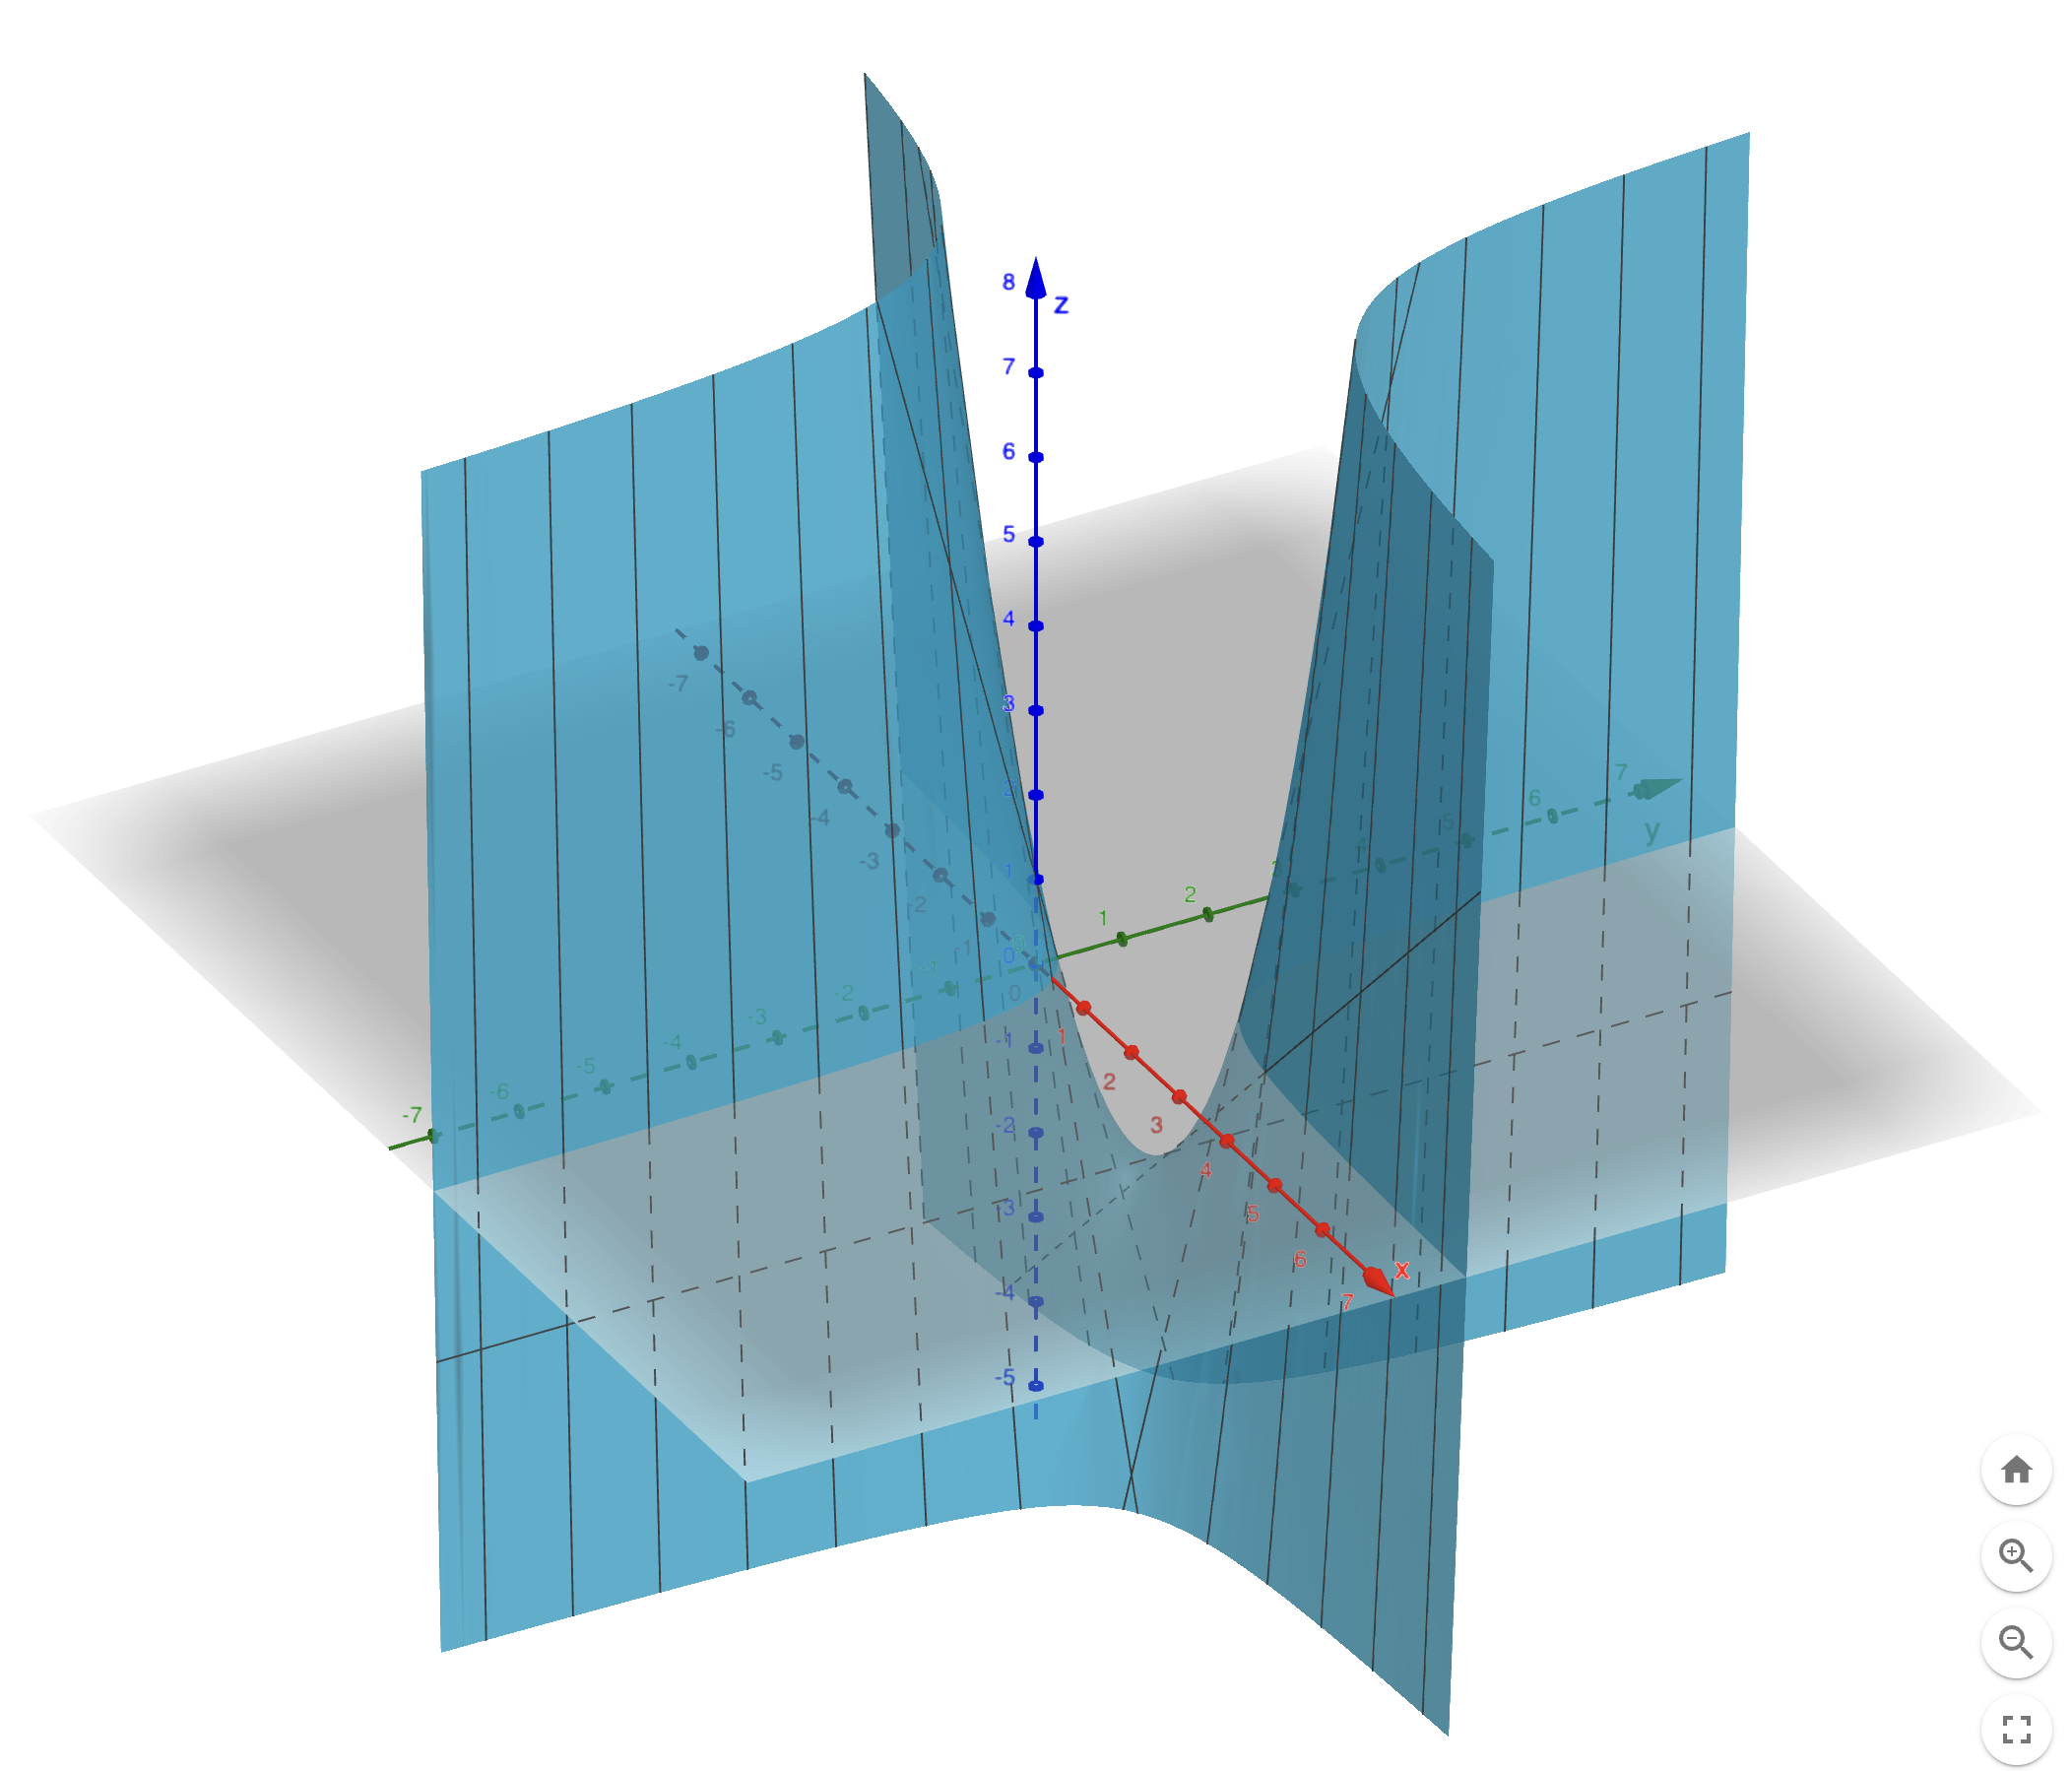
\includegraphics[scale=0.3]{assets/t_2_3.png} 
    \caption{$F_{y,x}= -x^3 + 4xy - 2y^2+1 \quad  Resultados \; coinciden$}
\end{figure}

\begin{figure}[h]
    \centering
    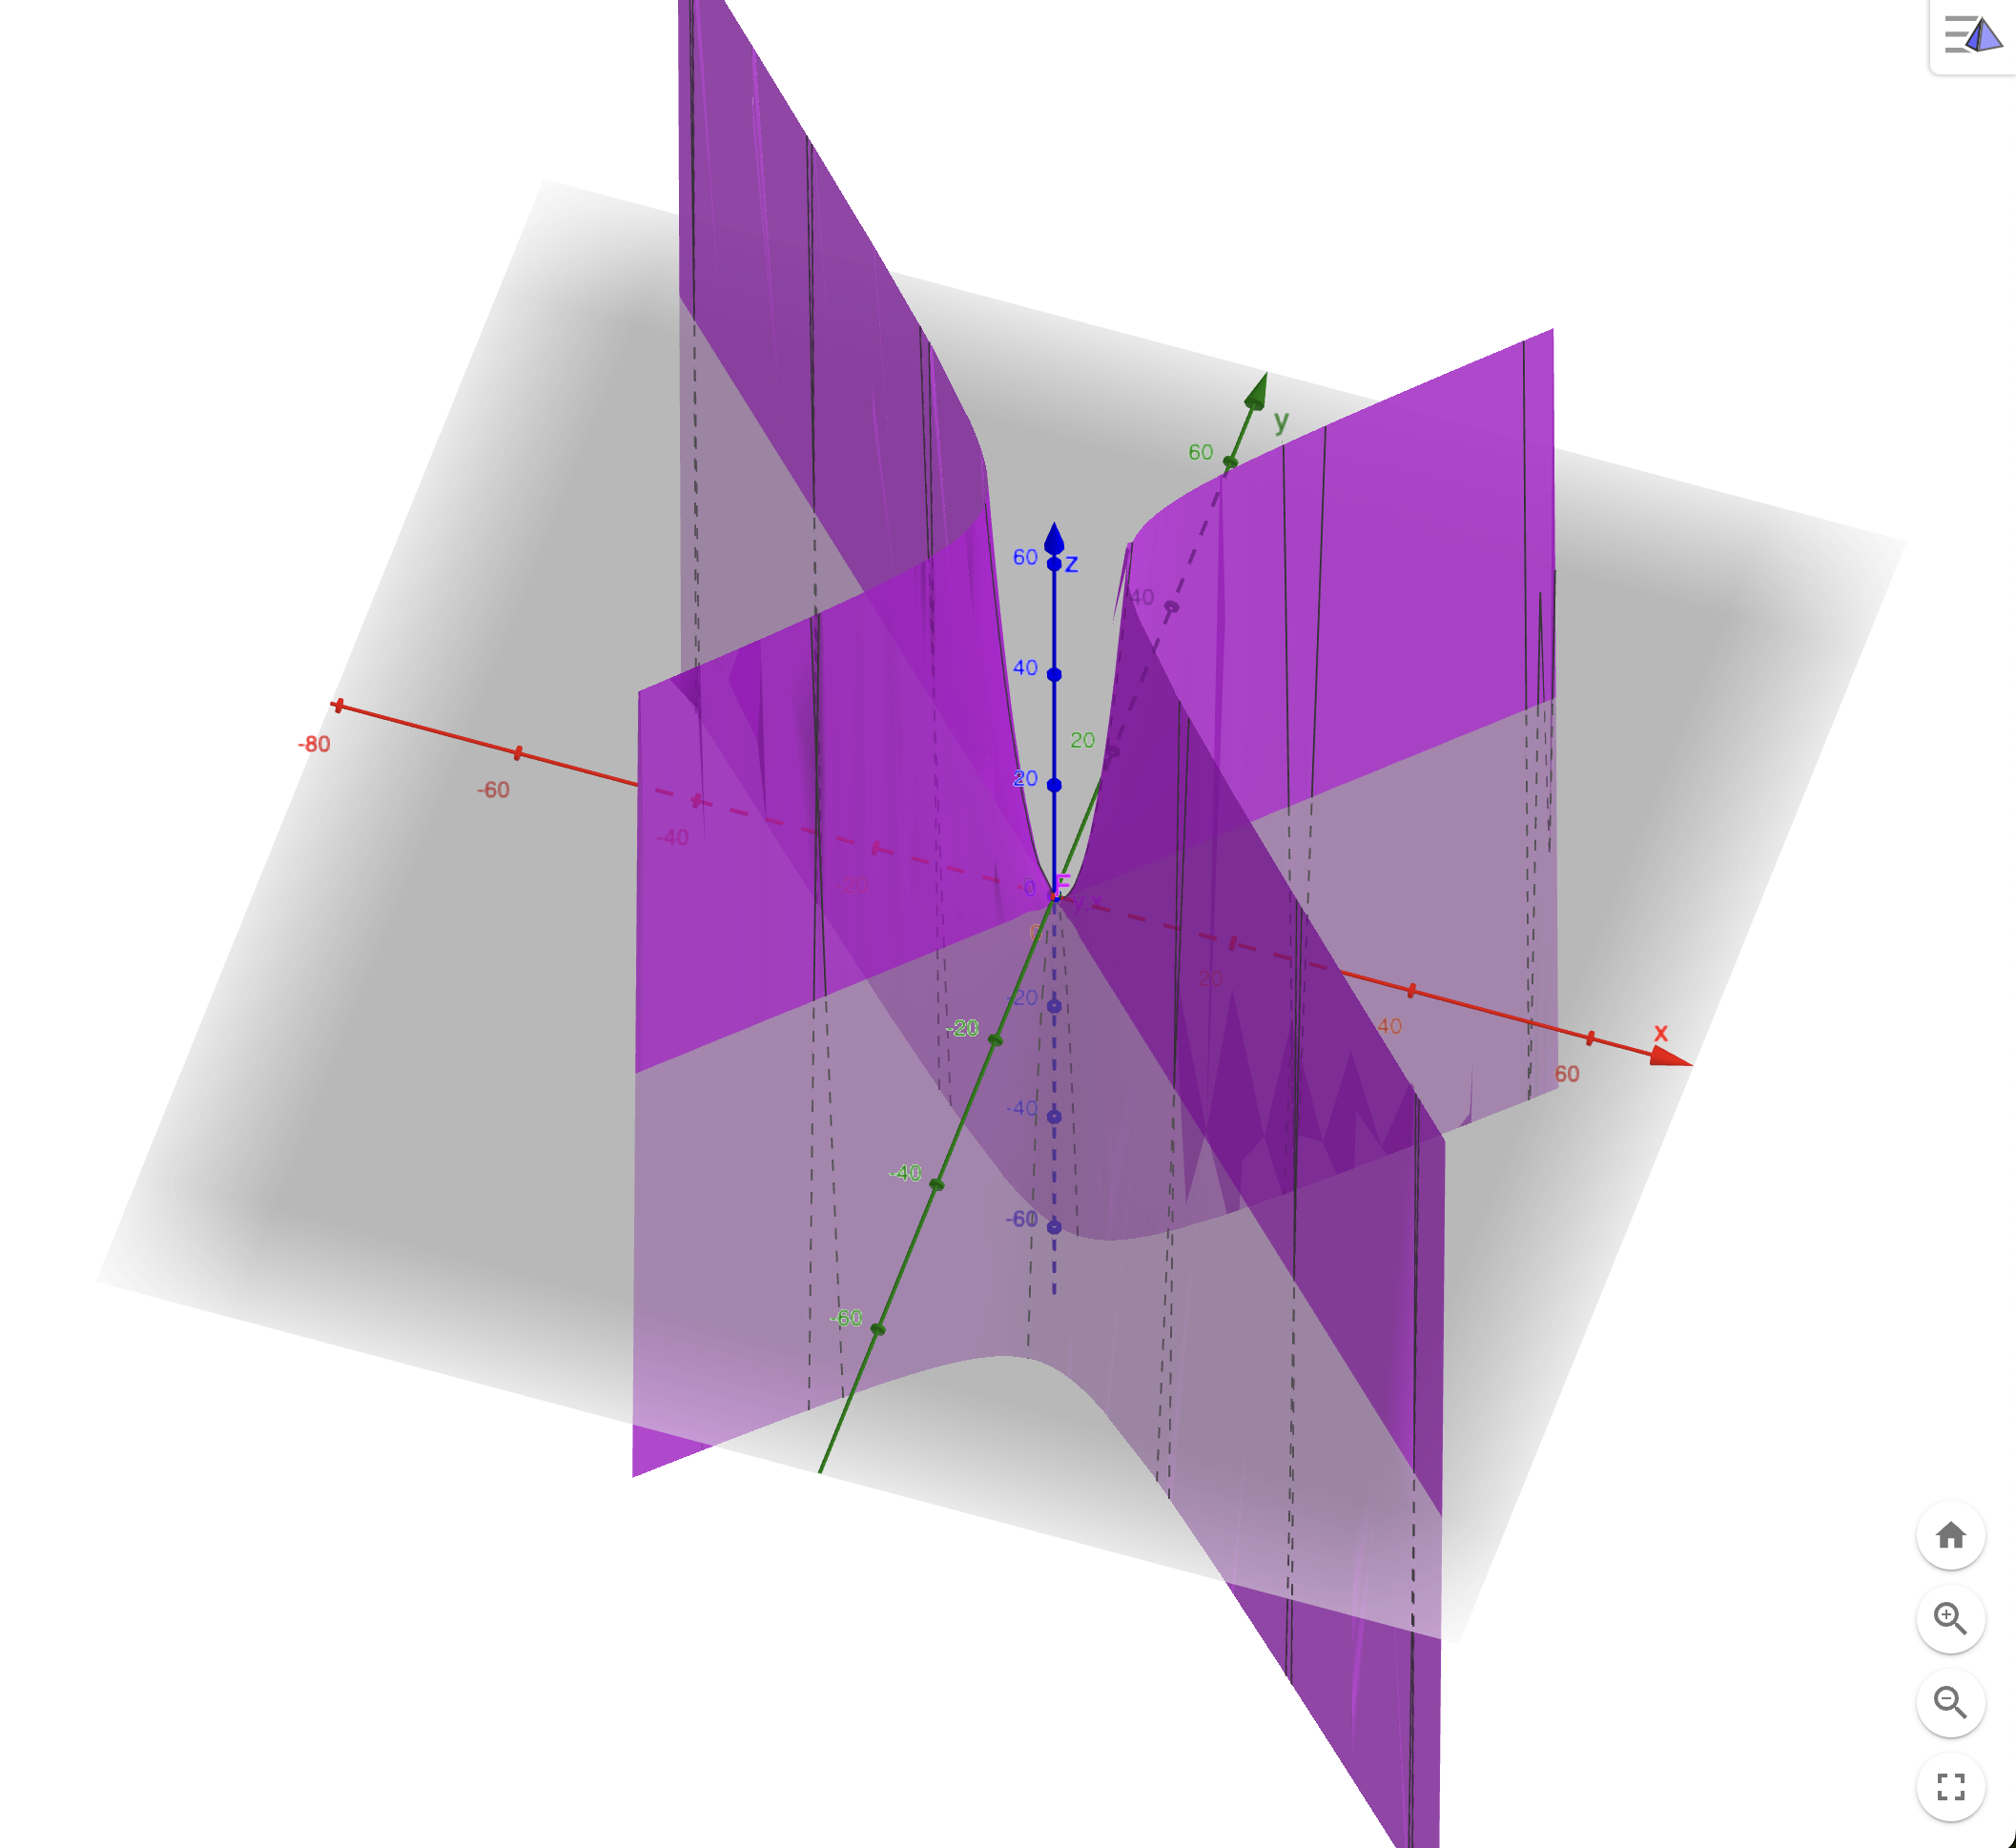
\includegraphics[scale=0.3]{assets/t_2_4.png} 
    \caption{$F_{y,x}= x^2-y^2-x-y \quad Resultados \; coinciden$}
\end{figure}

\begin{figure}[h]
    \centering 
    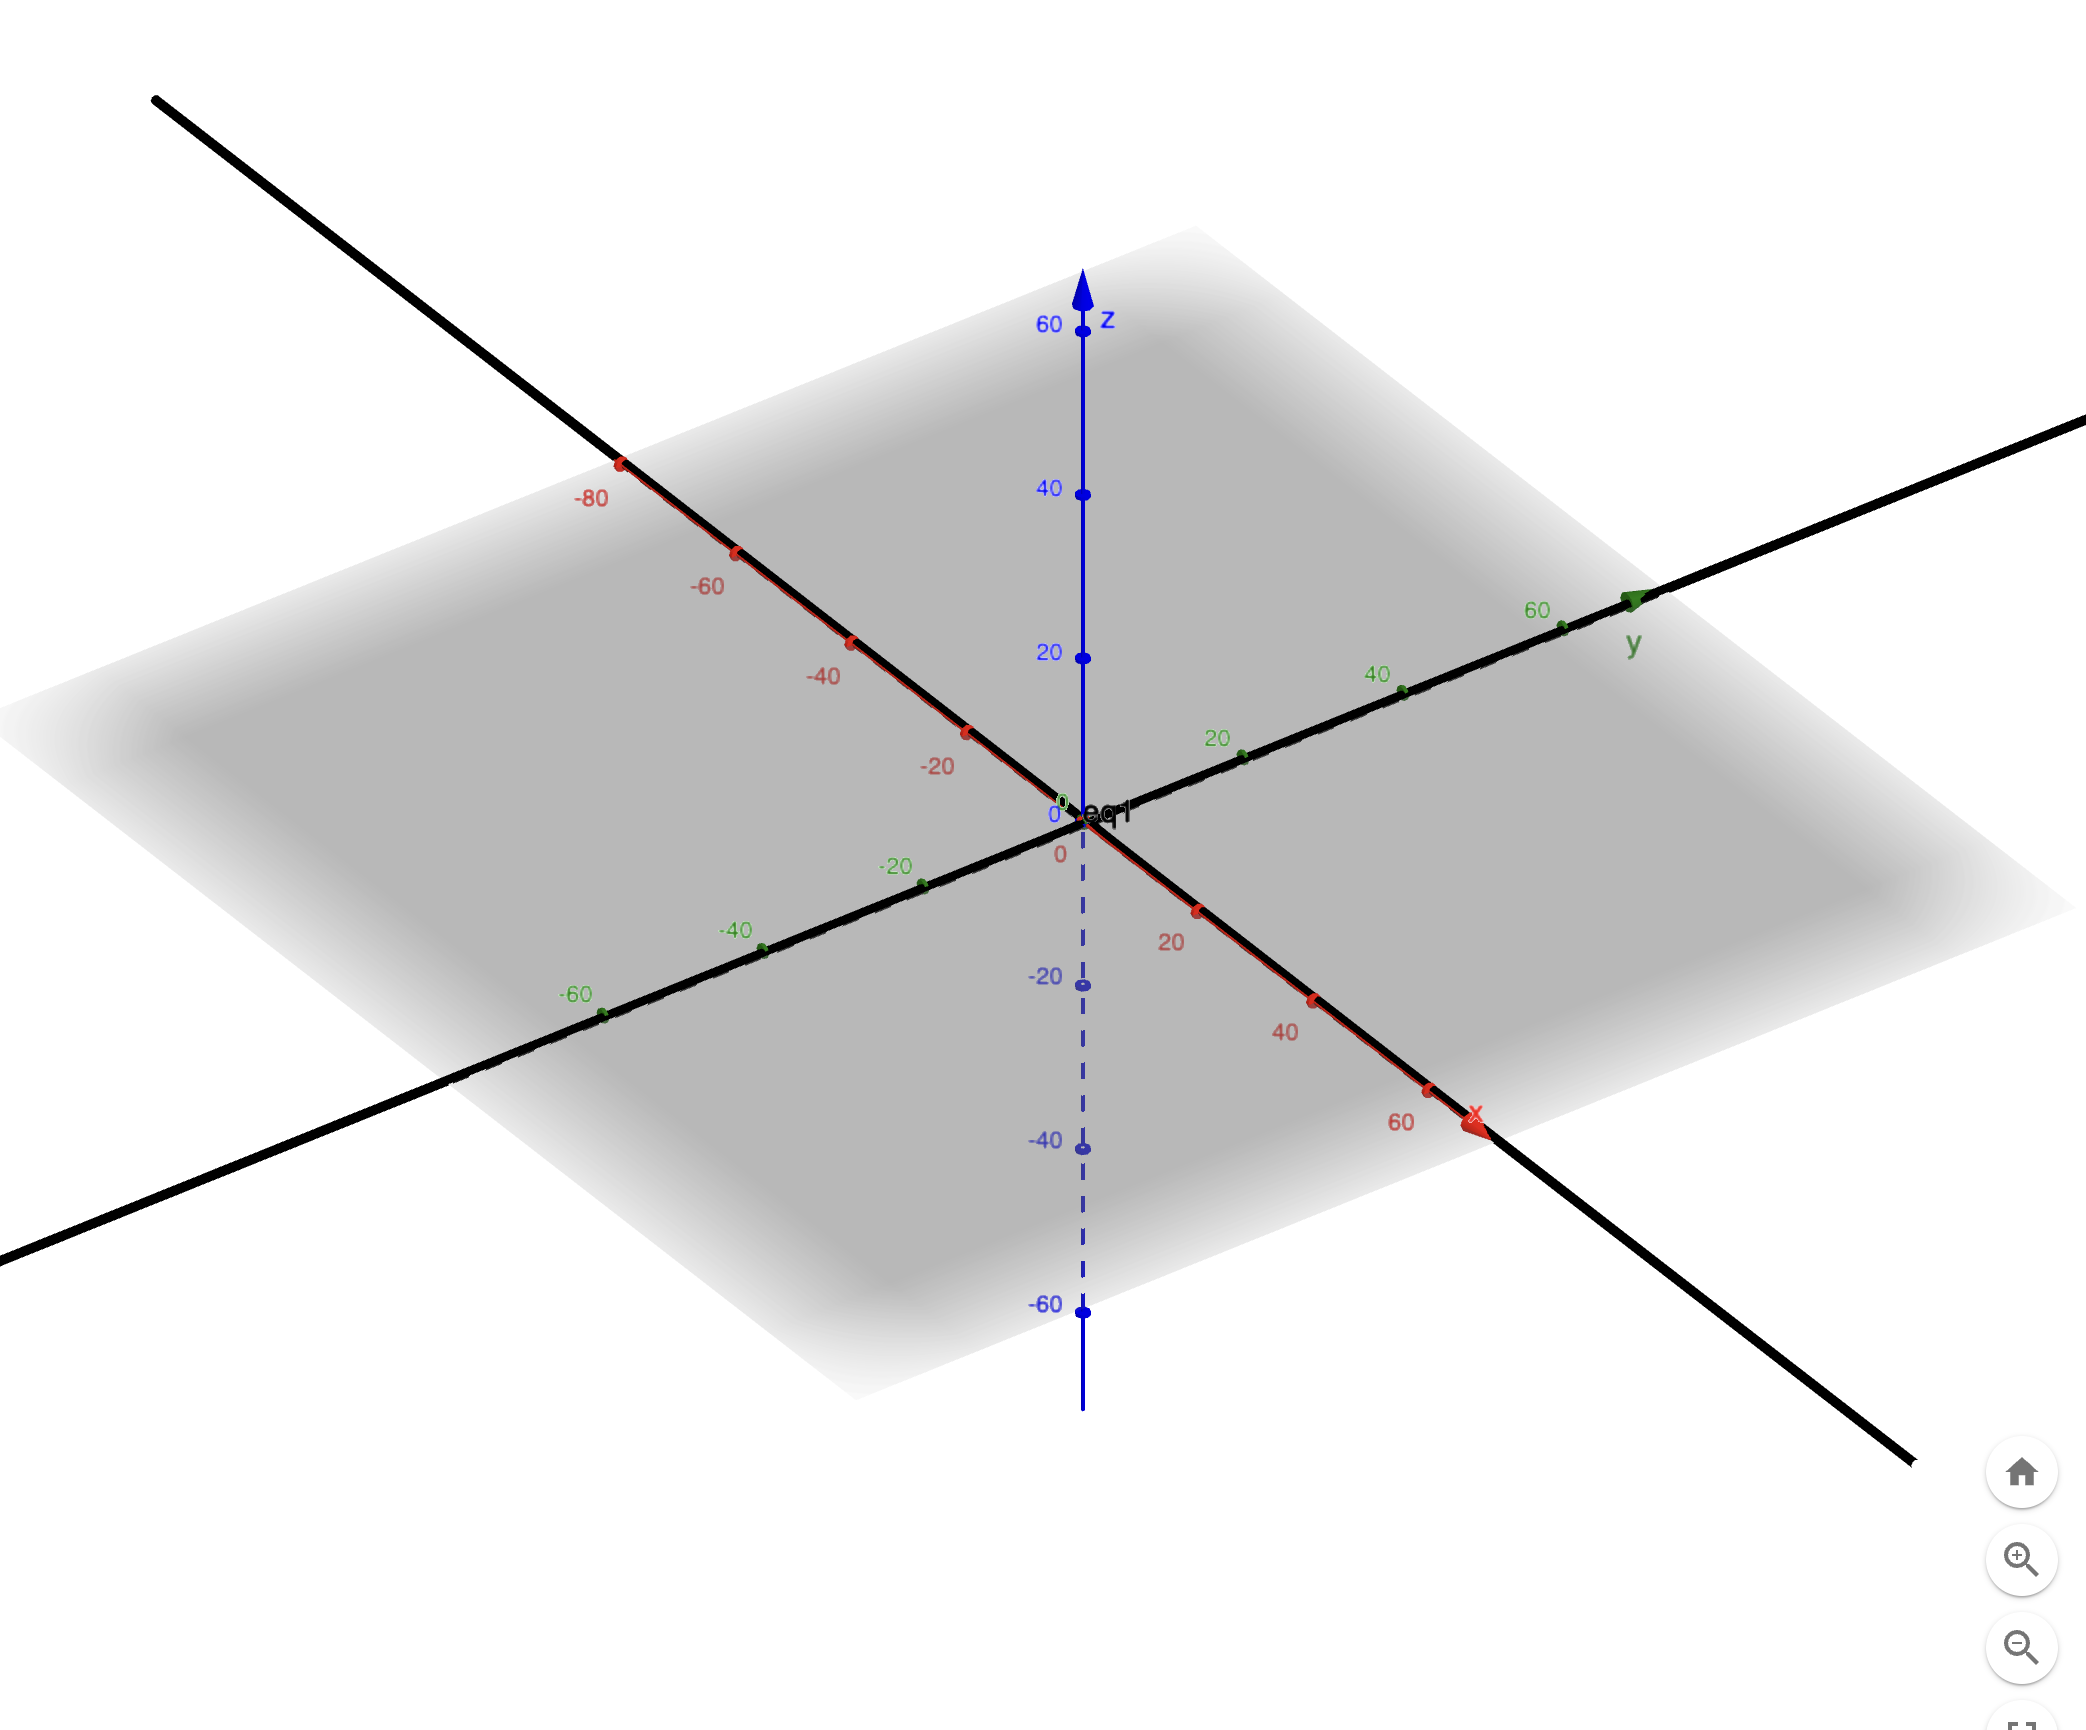
\includegraphics[scale=0.3]{assets/t_2_5.png} 
    \caption{$F_{y,x}= x^2-y^2-3xy \quad  Resultados \; coinciden$}
\end{figure}\\ 

\clearpage 

\item[ 4] ¿Cómo se calcula el plano tangente a una superficie? Busque y copie su defi- nición. Luego copie un ejemplo del libro donde se calcule un plano tangente (sección 14,4 del libro). Por último, calcule y grafique el plano tangente a:\\ 



\end{enumerate}	

\end{document}